% -*- root: apunte-metodos.tex -*-

\section{Normas matriciales, condicionamiento y estabilidad numérica}
\label{section:estabilidad}

A la hora de resolver problemas que involucran números reales utilizando la
computadora, siempre debe tenerse en cuenta que el abordaje de los mismos es
\textbf{numérico}, es decir, opera tan solo con aproximaciones de los números
reales, dentro de lo permitido por la aritmética finita de la computadora.
Esto produce, inevitablemente, errores de redondeo que pueden ocasionar pérdida
de exactitud en los resultados; por lo tanto, es importante tener cuidado en
evitar que dichos errores se propaguen de formas no deseadas.
En esta breve sección presentaremos algunos conceptos que serán útiles más
adelante para estudiar la forma en que distintos métodos pueden verse
afectados por errores de tipo numérico.

Una \textbf{norma matricial} es una extensión del concepto de norma vectorial
a matrices. Se trata de una función $\Phi$ que asigna a cada matriz un escalar
(para nosotros, siempre será un real) no negativo, y que se anula solamente en
la matriz $\mat{0}$; además, preserva el producto por escalares ($\Phi(
\lambda \cdot \mat{A}) = \lvert \lambda \rvert \cdot \Phi(\mat{A})$) y cumple
la desigualdad triangular ($\Phi(\mat{A} + \mat{B}) \leq \Phi(\mat{A}) +
\Phi(\mat{B})$).

Existen distintos tipos de normas matriciales. Nos interesaremos especialmente
en las \textbf{normas inducidas} por normas vectoriales. Si $\varphi$ es una
norma vectorial, definimos la norma matricial inducida por $\varphi$ como
\[ \Phi(\mat{A}) =
    \max \{ \varphi(\mat{A} \cdot \vec{v}) : \varphi(\vec{v}) = 1 \}. \]

Las siguientes dos propiedades valen para cualquier norma matricial inducida
$\Phi$:
\begin{enumerate}[label=(\roman*)]
\item $\Phi$ es \emph{submultiplicativa}: $\Phi(\mat{A} \cdot \mat{B}) \leq
    \Phi({\mat{A}}) \cdot \Phi(\mat{B})$.
\item $\Phi$ es \emph{consistente}: $\Phi(\mat{A} \cdot \vec{v}) \leq
    \Phi(\mat{A}) \cdot \varphi(\vec{v})$.
\end{enumerate}

A continuación se enumeran las tres normas vectoriales más comunes y sus
correspondientes normas matriciales.
\begin{itemize}
\item \textbf{Norma 1} o norma del taxista:
    \[ \lVert (v_1, \dots, v_n) \rVert_1
        = \lvert v_1 \rvert + \dots + \lvert v_n \rvert. \]

    La norma matricial inducida cumple que $\lVert \mat{A} \rVert_1
    = \max_{j} \lVert \col_j(\mat{A}) \rVert_1$.

\item \textbf{Norma 2} o norma euclídea:\footnote{En general,
    para $p \in \nats$, puede definirse la \emph{norma p}
    como $\lVert (v_1, \dots, v_n) \rVert_p
    = \sqrt[p]{(v_1)^p + \dots + (v_n)^p}$}
    \[ \lVert (v_1, \dots, v_n) \rVert_2
        = \sqrt{(v_1)^2 + \dots + (v_n)^2}. \]

\item \textbf{Norma infinito} o norma del máximo:
    \[ \lVert (v_1, \dots, v_n) \rVert_\infty
        = \max_{1 \leq i \leq n} \lvert v_i \rvert. \]

    La norma matricial inducida cumple que $\lVert \mat{A} \rVert_\infty
    = \max_{i} \lVert \fil_i(\mat{A}) \rVert_1$.
\end{itemize}

Las normas matriciales nos brindan herramientas para caracterizar sistemas de
ecuaciones problemáticos, donde pequeños errores numéricos pueden magnificarse
y producir soluciones considerablemente inexactas. Los sistemas que presentan
este tipo de inconvenientes se dice que están \textbf{mal condicionados}.

A modo de ejemplo, se puede pensar en un sistema de dos ecuaciones con dos
variables. Cada ecuación del sistema puede pensarse interpretarse como una
recta en el plano; una solución del sistema es un punto de intersección
entre ambas rectas. Consideremos un sistema como el de la figura
\ref{fig:sist-mal-condicionado}, donde las rectas son casi paralelas.

\begin{figure}[H]
\centering
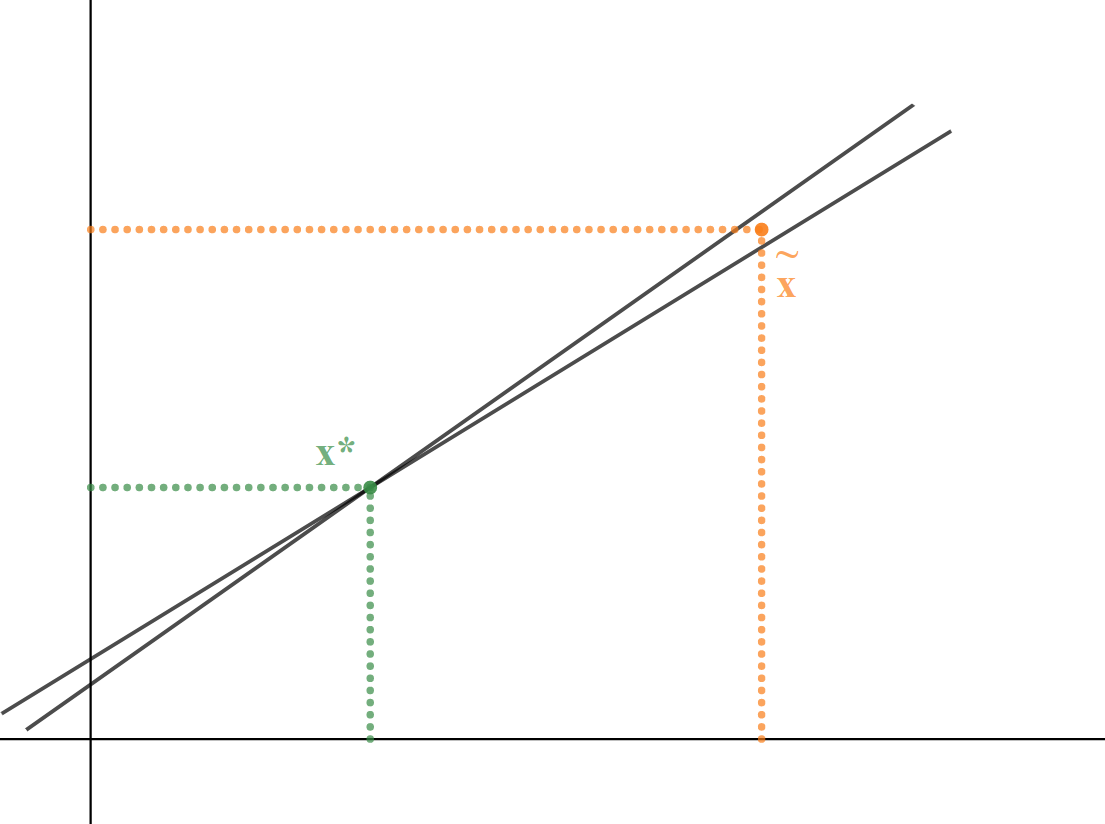
\includegraphics[width=10cm]{sist-mal-condicionado.png}
\caption{Sistema de ecuaciones mal condicionado.}
\label{fig:sist-mal-condicionado}
\end{figure}

Si bien el sistema tiene solución única $\vec{x^\ast}$, un pequeño error
numérico al resolver el sistema puede producir un resultado como
$\vec{\tilde x}$, donde las rectas también están muy próximas, pero que
se encuentra a una distancia considerable de $\vec{x^\ast}$.
Si consideramos la formulación matricial del sistema $\mat{A} \cdot \vec{x} =
\vec{b}$, entonces $\vec{\tilde x}$ es solución de un sistema $\mat{A} \cdot
\vec{x} = \vec{\tilde b}$ con $\vec{\tilde b}$ muy próximo a $\vec{b}$.
Es decir, un pequeño error en $\vec{b}$ se tradujo en un error
considerablemente más grande al obtener la solución $\vec{x^\ast}$.

Supongamos que tenemos una matriz $\mat{A}$ inversible. Considerando una norma
vectorial $\lVert \bullet \rVert$ cualquiera y su norma matricial inducida,
podemos demostrar las siguientes dos propiedades, que establecen una cota para
el error que puede generarse en la solución $\vec{x^\ast}$ (o error hacia
adelante) de un sistema $\mat{A} \cdot \vec{x} = \vec{b}$ a partir de un error
en la entrada $\vec{b}$ (o error hacia atrás):
\begin{enumerate}[label=(\roman*)]
\item $\lVert \vec{x^\ast} - \vec{\tilde x} \rVert \leq
    \lVert \vec{b} - \vec{\tilde b} \rVert \cdot
    \lVert \mat{A}^{-1} \rVert.$
\item $\dfrac{\lVert \vec{x^\ast} - \vec{\tilde x} \rVert}
        {\lVert \vec{x^\ast} \rVert} \leq
    \dfrac{\lVert \vec{b} - \vec{\tilde b} \rVert}
        {\lVert \vec{b} \rVert} \cdot
    \lVert \mat{A} \rVert \cdot
    \lVert \mat{A}^{-1} \rVert.$
\end{enumerate}

En la segunda propiedad se observa que el factor según el cual un error
relativo en las entradas puede magnificarse al producir un error relativo en
las soluciones es
\[ \kappa(\mat{A}) = \lVert \mat{A} \rVert \cdot \lVert \mat{A}^{-1} \rVert.
\]
A este valor se lo conoce como el \textbf{número de condición} de $\mat{A}$.
Para cualquier matriz, se cumple que $\kappa(\mat{A}) \geq \kappa(\mat{I})
= 1$. Si el número de condición de una matriz es alto, entonces la matriz
(y, en consecuencia, cualquier sistema de ecuaciones asociado a ella) está
mal condicionada.

Cabe destacar que estar bien o mal condicionado es una propiedad inherente del
sistema de ecuaciones que se busca resolver. Para un mismo sistema, distintos
algoritmos pueden ofrecer resultados de mayor o menos precisión, según el tipo
de operaciones que realizan y la magnitud de los errores que estas introducen
en los datos. A la propiedad de un algoritmo de manipular los datos sin
producir errores numéricos considerables se la denomina \textbf{estabilidad
numérica}.
